% Copyright 2004 by Till Tantau <tantau@users.sourceforge.net>.
%
% In principle, this file can be redistributed and/or modified under
% the terms of the GNU Public License, version 2.
%
% However, this file is supposed to be a template to be modified
% for your own needs. For this reason, if you use this file as a
% template and not specifically distribute it as part of a another
% package/program, I grant the extra permission to freely copy and
% modify this file as you see fit and even to delete this copyright
% notice. 

\documentclass{beamer}

% There are many different themes available for Beamer. A comprehensive
% list with examples is given here:
% http://deic.uab.es/~iblanes/beamer_gallery/index_by_theme.html
% You can uncomment the themes below if you would like to use a different
% one:
%\usetheme{AnnArbor}
%\usetheme{Antibes}
%\usetheme{Bergen}
%\usetheme{Berkeley}
%\usetheme{Berlin}
%\usetheme{Boadilla}
%\usetheme{boxes}
%\usetheme{CambridgeUS}
%\usetheme{Copenhagen}
%\usetheme{Darmstadt}
%\usetheme{default}
%\usetheme{Frankfurt}
%\usetheme{Goettingen}
%\usetheme{Hannover}
%\usetheme{Ilmenau}
%\usetheme{JuanLesPins}
%\usetheme{Luebeck}
\usetheme{Madrid}
%\usetheme{Malmoe}
%\usetheme{Marburg}
%\usetheme{Montpellier}
%\usetheme{PaloAlto}
%\usetheme{Pittsburgh}
%\usetheme{Rochester}
%\usetheme{Singapore}
%\usetheme{Szeged}
%\usetheme{Warsaw}

\newcommand{\link}[1]{{\color{blue}\href{#1}{#1}}}

\title[Strategic Subject Algorithm]{A regression analysis of the Strategic Subject Algorithm}

% A subtitle is optional and this may be deleted

\author{E. Sargent, esargent at hmc dot edu}
% - Give the names in the same order as the appear in the paper.
% - Use the \inst{?} command only if the authors have different
%   affiliation.

% - Use the \inst command only if there are several affiliations.
% - Keep it simple, no one is interested in your street address.

\date{November, 2019}
% - Either use conference name or its abbreviation.
% - Not really informative to the audience, more for people (including
%   yourself) who are reading the slides online

\subject{Theoretical Computer Science}
% This is only inserted into the PDF information catalog. Can be left
% out. 

% If you have a file called "university-logo-filename.xxx", where xxx
% is a graphic format that can be processed by latex or pdflatex,
% resp., then you can add a logo as follows:

% \pgfdeclareimage[height=0.5cm]{university-logo}{university-logo-filename}
% \logo{\pgfuseimage{university-logo}}

% Delete this, if you do not want the table of contents to pop up at
% the beginning of each subsection:
\AtBeginSubsection[]
{
  \begin{frame}<beamer>{Outline}
    \tableofcontents[currentsection,currentsubsection]
  \end{frame}
}

% Let's get started
\begin{document}

\begin{frame}
  \titlepage
\end{frame}

\begin{frame}{Outline}
  \tableofcontents
  % You might wish to add the option [pausesections]
\end{frame}

% Section and subsections will appear in the presentation overview
% and table of contents.
\section{Introduction}

\subsection{History of the SSA}

\begin{frame}{History of the SSA}
  \begin{itemize}
  \item {
    Developed at the Illinois Institute of Technology in 2013, in cooperation with the Chicago Police Department.
  }
  \item {
   Ranked hundreds of thousands of Chicagoans based on their estimated likelihood of involvement in a shooting, as either as a victim or a perpetrator \cite{nyt}.
  }
  \item {
    Discontinued in 2019 in favor of the Crime Reduction Victimization Model (CVRM).
  }
  \end{itemize}
\end{frame}

\subsection{Previous reporting on the SSA}

% You can reveal the parts of a slide one at a time
% with the \pause command:
\begin{frame}{Previous reporting on the SSA}
  \begin{itemize}
  \item {
    Chicago Sun Times, 2017
    \begin{itemize}
        \item FOIA request, legal battle, release of 2017 version of Strategic Subject List (SSL)
    \end{itemize}
  }
  \item {
    New York Times, 2017
    \begin{itemize}
        \item linear regression on SSL scores
        \item score mostly ($R^2 = 89$\%) reflects a person's age
    \end{itemize}
  }
  \item {   
    Upturn, 2017
    \begin{itemize}
        \item linear regression on SSL scores
        \item discussion of the customs notification program
        %\ 'The CPD itself describes Custom Notifications as “a process that identifies potential criminal actors and victims associated with the continuum of violence.  Once identified,  the individual is notified of the consequences that will result should violent activity continue.” Between 2013 and 2016, the CPD is reported to have made over 1,400 of these visits.'%\
    \end{itemize}
  }
  % You can also specify when the content should appear
  % by using <n->:
  \end{itemize}
\end{frame}

\section{Exploratory Data Analysis}

\subsection{The SSL}

\begin{frame}{The SSL}
\begin{itemize}
    \item Most recent version: Dec. 7, 2017
    \item 398,684 subjects
    \item 53  fields
    \begin{itemize}
        \item 8  predictor  fields,  which  the  CPD  claims  are  the  only  fields used  in  computing  the  SSL  Score
        \item  44  other  fields  including  variables  like  race,  sex,  and geographical location,  and SSL Score itself
    \end{itemize} 
    
\end{itemize}
\end{frame}

\subsection{Predictors and their distributions}

\begin{frame}{Predictors and their distributions}
\begin{center}
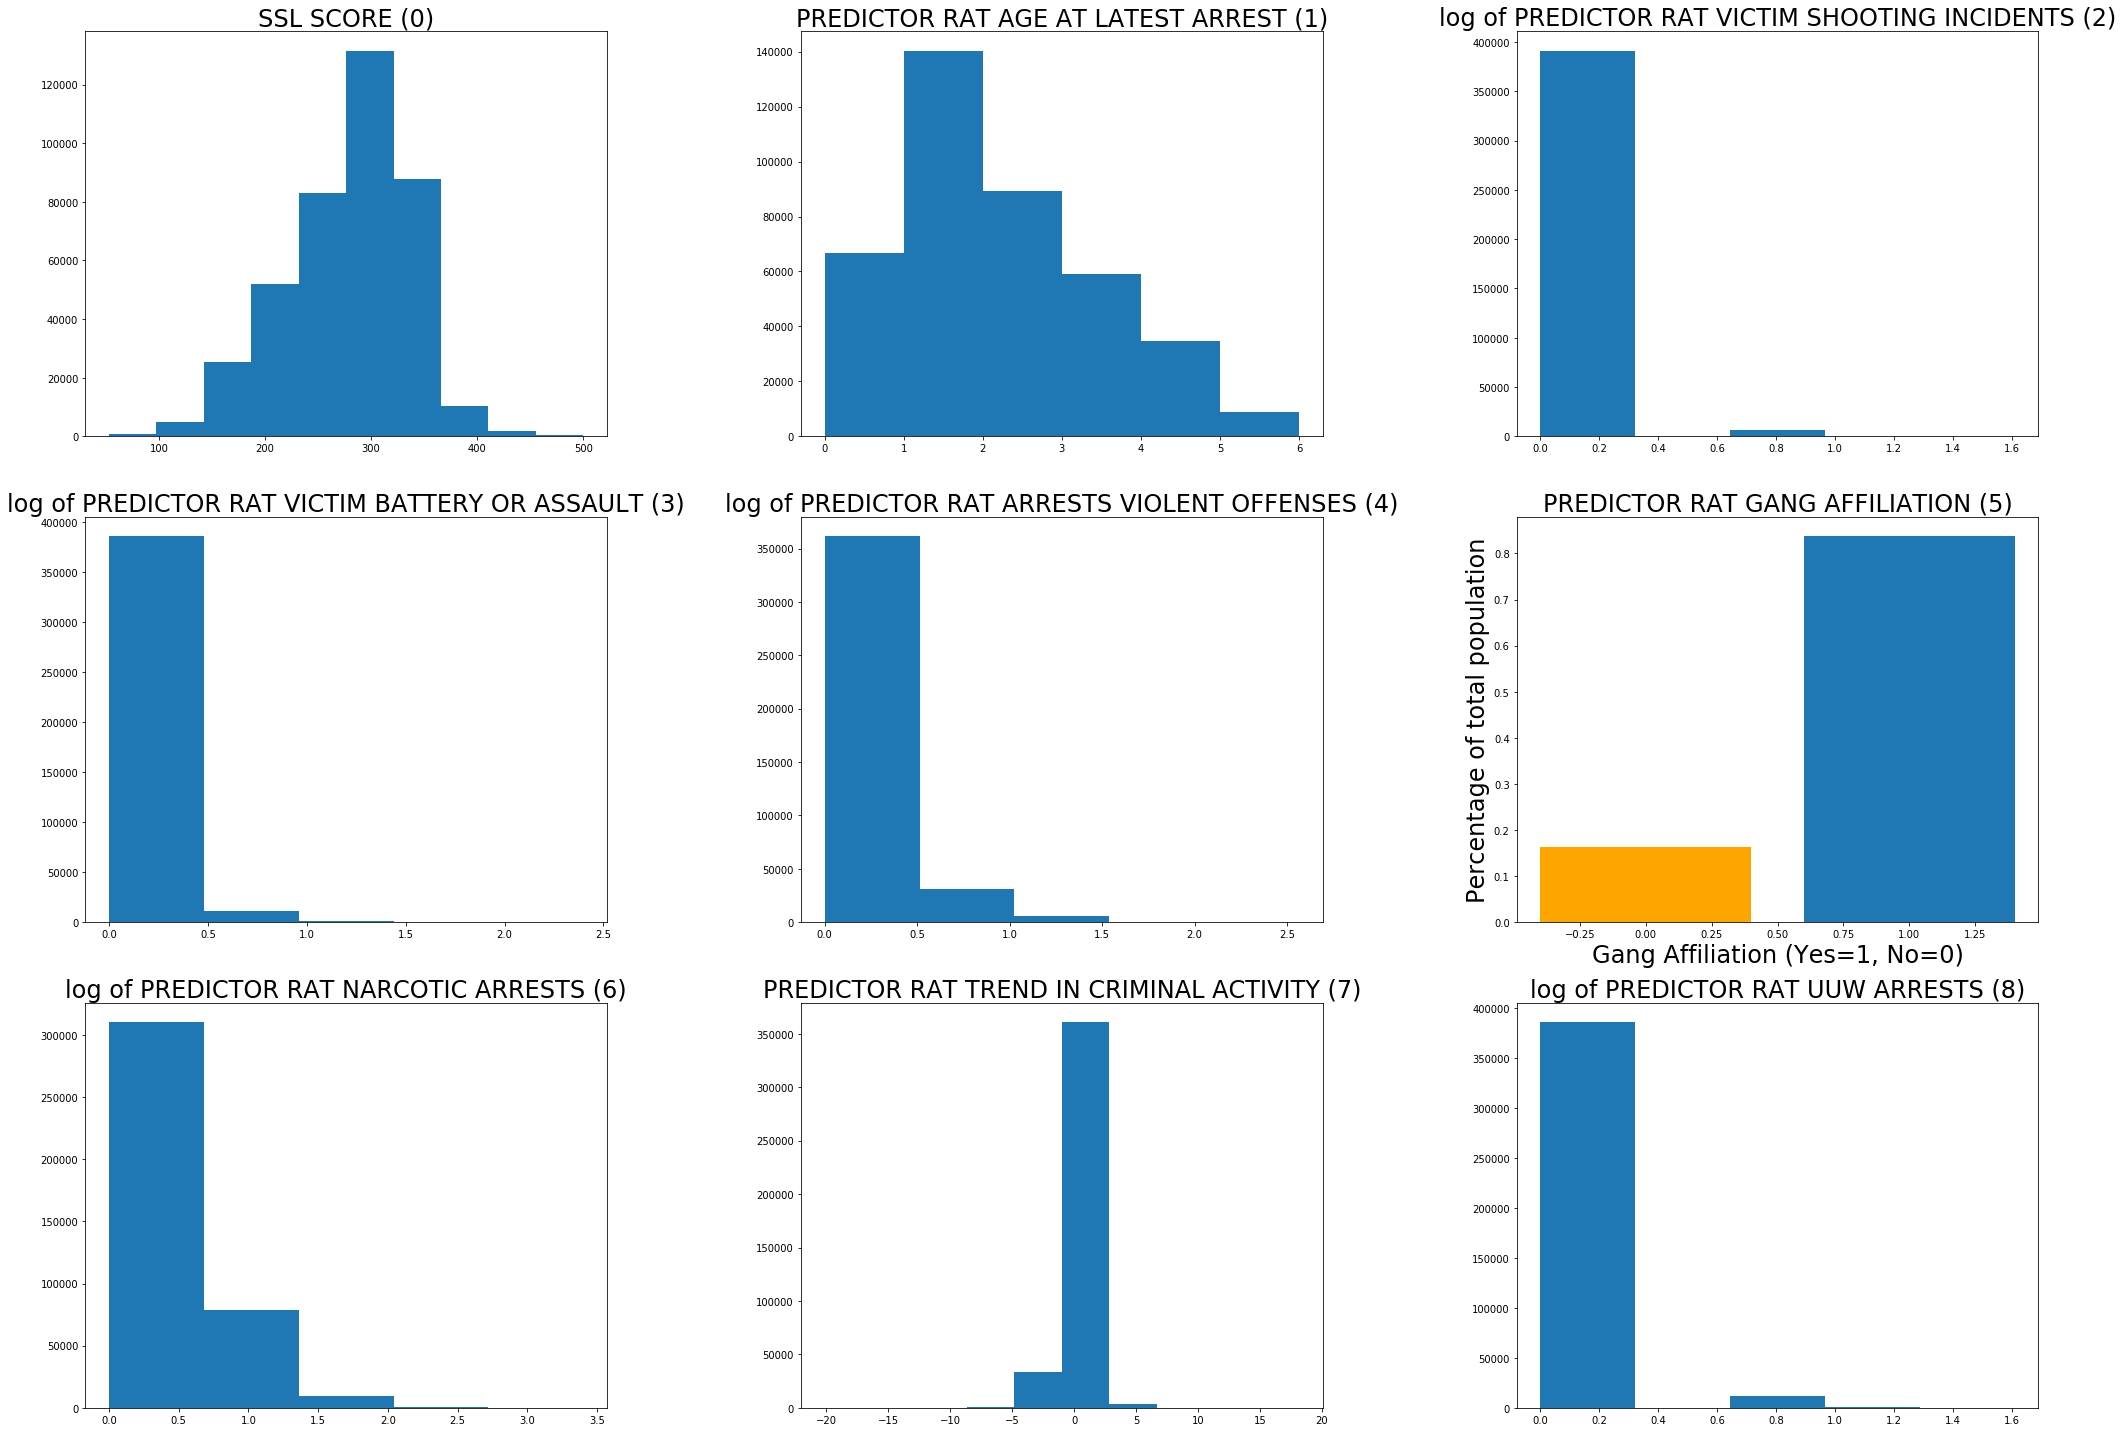
\includegraphics[scale=.15]{distribs.png}
\end{center}
\end{frame}

\subsection{The predictor \texttt{TREND IN CRIMINAL ACTIVITY}}

\begin{frame}{Predictors and their distributions}
\begin{itemize}
    \item Unknown distribution (many outliers)
    \item Possibly computed from missing data
\end{itemize}

\begin{center}
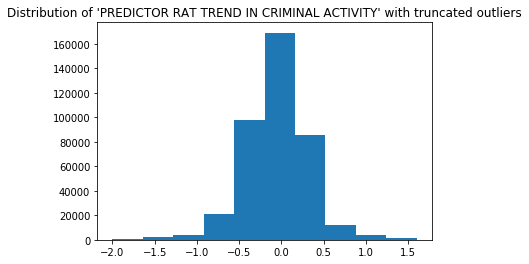
\includegraphics[scale=.4]{trends.png}
\end{center}
\end{frame}

\subsection{Location, race, and gender}
\begin{frame}{Location}
\begin{itemize}
    \item lat/long of most recent arrest for only 224,235 subjects, or 56.24\% of the total.
\end{itemize}
\begin{center}
    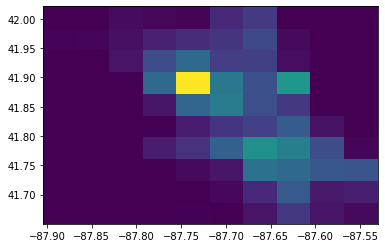
\includegraphics[scale=.5]{locations.png}
\end{center}
\end{frame}

\begin{frame}{Sex and race}
\begin{itemize}
    \item Between-group differences are slight, but statistically significant
\end{itemize}
\begin{center}
    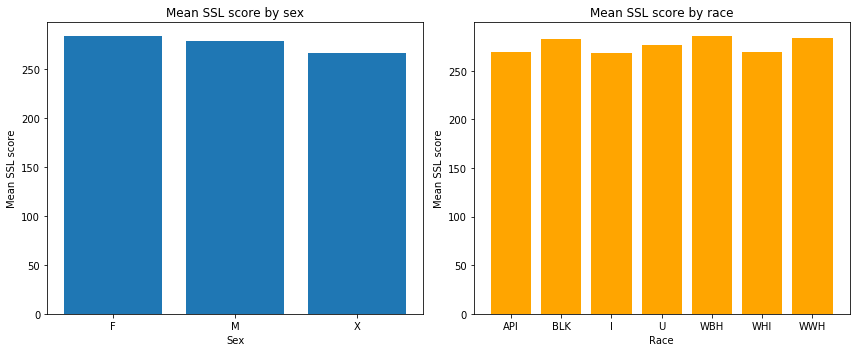
\includegraphics[scale=.4]{race.png}
\end{center}
\end{frame}

\section{Models}
\subsection{Modeling SSL score}

\begin{frame}{Modeling SSL score}
\begin{itemize}
    \item best-performing model: \texttt{xgboost}
\end{itemize}
\begin{table}[h!]
\centering
\begin{tabular}{||c c c||}
 \hline
 Model & RMSE & Cross-validated\\ [0.5ex] 
 \hline\hline
\texttt{OLS} (age only) & $19.55$ & No\\
\texttt{OLS} & $12.97$ & No\\
\texttt{OLS} w/ polynomial features (deg $\leq 3$) & $12.48$ & No\\
\texttt{Random Forests} & 12.47 & Yes\\
\texttt{XGBoost} & 12.38 & No\\
 \hline
\end{tabular}
\label{table:2}
\end{table}
\end{frame}

\begin{frame}{Modeling SSL score (cont.)}
\begin{itemize}
    \item Age is by far the most important feature
\end{itemize}
\begin{center}
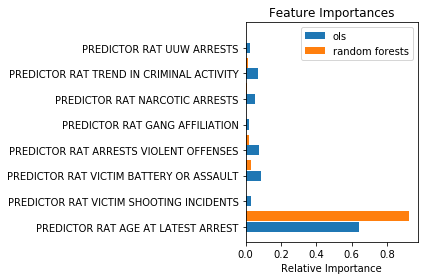
\includegraphics[scale=.6]{feature_importances.png}
\end{center}
\end{frame}

\begin{frame}{Modeling SSL score (cont.)}
\begin{itemize}
    \item Narcotic arrests, the second principal component of a principal component decomposition of the predictors, is not an input to the CVRM.
\end{itemize}
\begin{center}
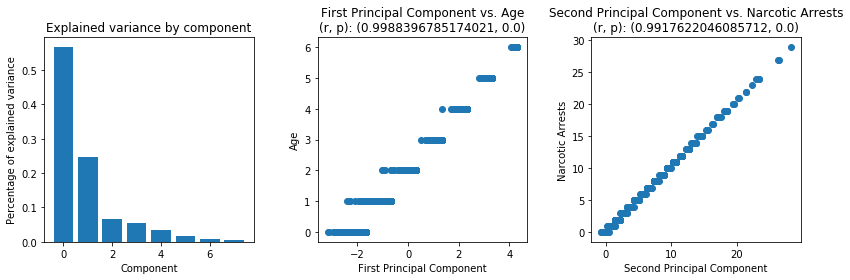
\includegraphics[scale=.4]{pca.png}
\end{center}
\end{frame}


\subsection{Modeling \texttt{TREND}}

\begin{frame}{Modeling \texttt{TREND}}
\begin{itemize}
    \item Per \cite{factsheet}, "the 'trend' variable is the slope of a line obtained by a least-squares fit to the individual’s numbers of arrests each year for the past four years."
    \item Data to compute this is missing
    \item Two approximations with our incomplete data:
        \begin{itemize}
            \item 0 substitution
            \item slope substitution
        \end{itemize}
\end{itemize}
\end{frame}

\begin{frame}{Modeling \texttt{TREND} (cont.)}
\begin{table}[h!]
\centering
\begin{tabular}{||c c c c||}
 \hline
 Model & Substitution & RMSE & Cross-validated\\ [0.5ex] 
 \hline\hline
Random model & n/a & $0.5726$ & No\\
\texttt{OLS} & 0 & $0.32786$ & No\\
\texttt{OLS} & slope & $0.3135$ & No\\
\texttt{OLS} w/ polynomial features & 0 & $0.2895$ & No\\
\texttt{OLS} w/ polynomial features & slope & $0.2843$ & No\\
Random forests & 0 & $0.2832$ & Yes\\
Random forests & slope & $0.2848$ & Yes\\
 \hline
\end{tabular}
\label{table:2}
\end{table}
\end{frame}

% Placing a * after \section means it will not show in the
% outline or table of contents.

% All of the following is optional and typically not needed. 
\appendix
\section<presentation>*{\appendixname}
\subsection<presentation>*{For Further Reading}

\begin{frame}[allowframebreaks]
  \frametitle<presentation>{For Further Reading}
    
\begin{thebibliography}{9}
\bibitem{nyt} 
J. Asher and R. Arthur, "Inside the Algorithm That Tries to Predict Gun Violence in Chicago."
New York Times, 13 June 2017;
\link{https://www.nytimes.com/2017/06/13/upshot/what-an-algorithm-reveals-about-life-on-chicagos-high-risk-list.html}

\bibitem{upturn} 
B. Posadas, "How strategic is Chicago’s 'Strategic Subjects List'? Upturn investigates."
Medium, 22 June 2017;
\link{https://medium.com/equal-future/how-strategic-is-chicagos-strategic-subjects-list-upturn-investigates-9e5b4b235a7c}

\bibitem{data} 
Chicago Data Portal, 7 December 2017;
\link{https://data.cityofchicago.org/Public-Safety/Strategic-Subject-List/4aki-r3np}

\bibitem{factsheet}
"Crime and Victimization Risk Model (CVRM)." Illinois Insitute of Technology, n.d.;
\link{https://home.chicagopolice.org/wp-content/uploads/2019/01/FACT-SHEET-Crime-and-Victimization-Risk-Model-1.pdf}

\bibitem{directive} 
"SUBJECT ASSESSMENT AND INFORMATION DASHBOARD (SAID)." Chicago Police Department, 09 January 2019.
\link{http://directives.chicagopolice.org/directives/data/a7a57b85-155e9f4b-50c15-5e9f-7742e3ac8b0ab2d3.html?hl=true}

\bibitem{crime} 
"Crime in Chicago: Explore your community." Chicago Tribune, 01 April 2019.
\link{https://www.chicagotribune.com/news/ct-crime-in-chicago-20171114-storygallery.html}

\bibitem{lawyer}
"Gun Charge in Illinois FAQs." Robert J. Callahan: Chicago Criminal Defense Attorney, n.d.; \link{https://www.defenselawyersite.com/gun-charge-in-illinois-faqs/}

\bibitem{sun-times}
M. Dumke and F. Main, "A look inside the watch list Chicago police fought to keep secret." Chicago Sun Times, 18 May 2017.
\link{https://chicago.suntimes.com/2017/5/18/18386116/a-look-inside-the-watch-list-chicago-police-fought-to-keep-secret}

\end{thebibliography}
\end{frame}


\end{document}


